\pgfdeclareplotmark{cross} {
\pgfpathmoveto{\pgfpoint{-0.3\pgfplotmarksize}{\pgfplotmarksize}}
\pgfpathlineto{\pgfpoint{+0.3\pgfplotmarksize}{\pgfplotmarksize}}
\pgfpathlineto{\pgfpoint{+0.3\pgfplotmarksize}{0.3\pgfplotmarksize}}
\pgfpathlineto{\pgfpoint{+1\pgfplotmarksize}{0.3\pgfplotmarksize}}
\pgfpathlineto{\pgfpoint{+1\pgfplotmarksize}{-0.3\pgfplotmarksize}}
\pgfpathlineto{\pgfpoint{+0.3\pgfplotmarksize}{-0.3\pgfplotmarksize}}
\pgfpathlineto{\pgfpoint{+0.3\pgfplotmarksize}{-1.\pgfplotmarksize}}
\pgfpathlineto{\pgfpoint{-0.3\pgfplotmarksize}{-1.\pgfplotmarksize}}
\pgfpathlineto{\pgfpoint{-0.3\pgfplotmarksize}{-0.3\pgfplotmarksize}}
\pgfpathlineto{\pgfpoint{-1.\pgfplotmarksize}{-0.3\pgfplotmarksize}}
\pgfpathlineto{\pgfpoint{-1.\pgfplotmarksize}{0.3\pgfplotmarksize}}
\pgfpathlineto{\pgfpoint{-0.3\pgfplotmarksize}{0.3\pgfplotmarksize}}
\pgfpathclose
\pgfusepathqstroke
}
\pgfdeclareplotmark{cross*} {
\pgfpathmoveto{\pgfpoint{-0.3\pgfplotmarksize}{\pgfplotmarksize}}
\pgfpathlineto{\pgfpoint{+0.3\pgfplotmarksize}{\pgfplotmarksize}}
\pgfpathlineto{\pgfpoint{+0.3\pgfplotmarksize}{0.3\pgfplotmarksize}}
\pgfpathlineto{\pgfpoint{+1\pgfplotmarksize}{0.3\pgfplotmarksize}}
\pgfpathlineto{\pgfpoint{+1\pgfplotmarksize}{-0.3\pgfplotmarksize}}
\pgfpathlineto{\pgfpoint{+0.3\pgfplotmarksize}{-0.3\pgfplotmarksize}}
\pgfpathlineto{\pgfpoint{+0.3\pgfplotmarksize}{-1.\pgfplotmarksize}}
\pgfpathlineto{\pgfpoint{-0.3\pgfplotmarksize}{-1.\pgfplotmarksize}}
\pgfpathlineto{\pgfpoint{-0.3\pgfplotmarksize}{-0.3\pgfplotmarksize}}
\pgfpathlineto{\pgfpoint{-1.\pgfplotmarksize}{-0.3\pgfplotmarksize}}
\pgfpathlineto{\pgfpoint{-1.\pgfplotmarksize}{0.3\pgfplotmarksize}}
\pgfpathlineto{\pgfpoint{-0.3\pgfplotmarksize}{0.3\pgfplotmarksize}}
\pgfpathclose
\pgfusepathqfillstroke
}
\pgfdeclareplotmark{newstar} {
\pgfpathmoveto{\pgfqpoint{0pt}{\pgfplotmarksize}}
\pgfpathlineto{\pgfqpointpolar{44}{0.5\pgfplotmarksize}}
\pgfpathlineto{\pgfqpointpolar{18}{\pgfplotmarksize}}
\pgfpathlineto{\pgfqpointpolar{-20}{0.5\pgfplotmarksize}}
\pgfpathlineto{\pgfqpointpolar{-54}{\pgfplotmarksize}}
\pgfpathlineto{\pgfqpointpolar{-90}{0.5\pgfplotmarksize}}
\pgfpathlineto{\pgfqpointpolar{234}{\pgfplotmarksize}}
\pgfpathlineto{\pgfqpointpolar{198}{0.5\pgfplotmarksize}}
\pgfpathlineto{\pgfqpointpolar{162}{\pgfplotmarksize}}
\pgfpathlineto{\pgfqpointpolar{134}{0.5\pgfplotmarksize}}
\pgfpathclose
\pgfusepathqstroke
}
\pgfdeclareplotmark{newstar*} {
\pgfpathmoveto{\pgfqpoint{0pt}{\pgfplotmarksize}}
\pgfpathlineto{\pgfqpointpolar{44}{0.5\pgfplotmarksize}}
\pgfpathlineto{\pgfqpointpolar{18}{\pgfplotmarksize}}
\pgfpathlineto{\pgfqpointpolar{-20}{0.5\pgfplotmarksize}}
\pgfpathlineto{\pgfqpointpolar{-54}{\pgfplotmarksize}}
\pgfpathlineto{\pgfqpointpolar{-90}{0.5\pgfplotmarksize}}
\pgfpathlineto{\pgfqpointpolar{234}{\pgfplotmarksize}}
\pgfpathlineto{\pgfqpointpolar{198}{0.5\pgfplotmarksize}}
\pgfpathlineto{\pgfqpointpolar{162}{\pgfplotmarksize}}
\pgfpathlineto{\pgfqpointpolar{134}{0.5\pgfplotmarksize}}
\pgfpathclose
\pgfusepathqfillstroke
}
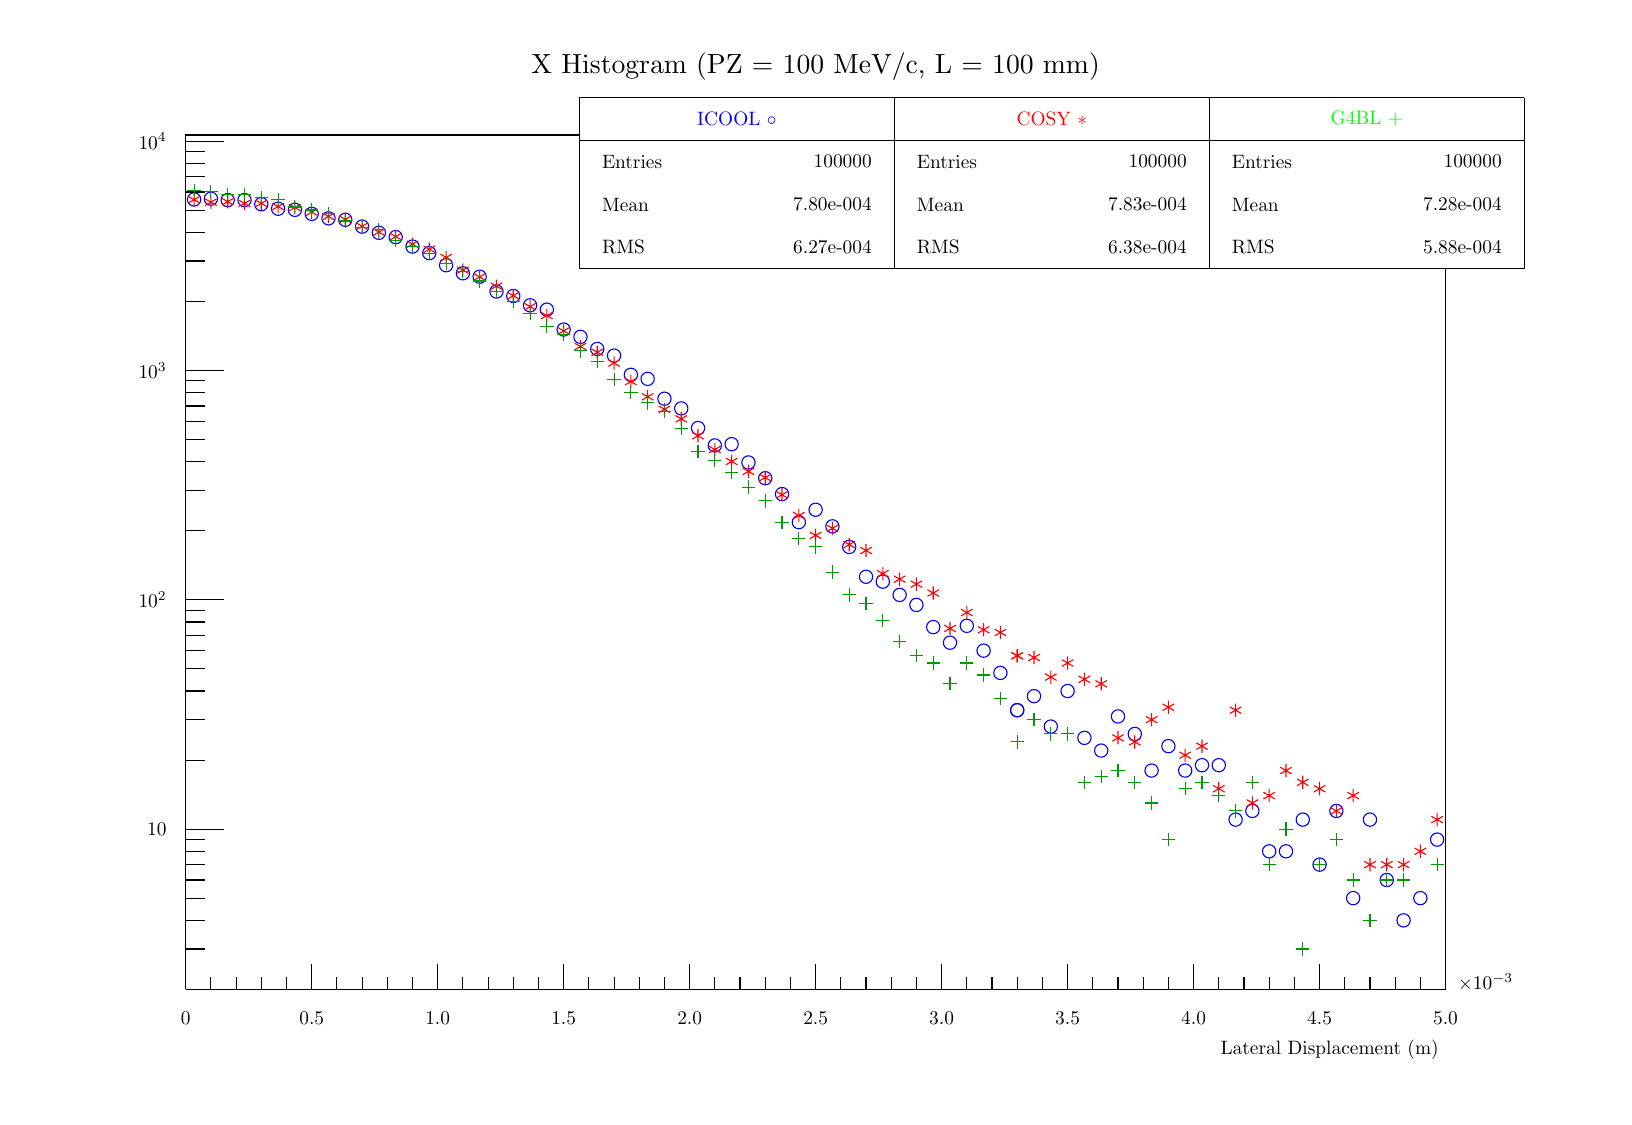
\begin{tikzpicture}
\definecolor{c}{rgb}{1,1,1};
\draw [color=c, fill=c] (0,0) rectangle (20,13.5632);
\draw [color=c, fill=c] (2,1.35632) rectangle (18,12.2069);
\definecolor{c}{rgb}{0,0,0};
\draw [c] (2,1.35632) -- (2,12.2069) -- (18,12.2069) -- (18,1.35632) -- (2,1.35632);
\definecolor{c}{rgb}{1,1,1};
\draw [color=c, fill=c] (2,1.35632) rectangle (18,12.2069);
\definecolor{c}{rgb}{0,0,0};
\draw [c] (2,1.35632) -- (2,12.2069) -- (18,12.2069) -- (18,1.35632) -- (2,1.35632);
\definecolor{c}{rgb}{0,0,1};
\foreach \P in
 {(2.10667,11.3888),(2.32,11.3986),(2.53333,11.3804),(2.74667,11.3806),(2.96,11.3281),(3.17333,11.2708),(3.38667,11.2568),(3.6,11.2053),(3.81333,11.1484),(4.02667,11.1299),(4.24,11.0434),(4.45333,10.9652),(4.66667,10.91),(4.88,10.7901),(5.09333,10.70
69),(5.30667,10.5534),(5.52,10.4509),(5.73333,10.4073),(5.94667,10.2193),(6.16,10.1625),(6.37333,10.0445),(6.58667,9.98877),(6.8,9.7364),(7.01333,9.64331),(7.22667,9.48993),(7.44,9.40564),(7.65333,9.16123),(7.86667,9.10998),(8.08,8.858),(8.29333,8.73
459),(8.50667,8.4857),(8.72,8.26453),(8.93333,8.28054),(9.14667,8.04834),(9.36,7.84857),(9.57333,7.64674),(9.78667,7.29014),(10,7.44811),(10.2133,7.23681),(10.4267,6.97558),(10.64,6.59674),(10.8533,6.53502),(11.0667,6.36613),(11.28,6.23954),(11.4933,
5.9573),(11.7067,5.75954),(11.92,5.97383),(12.1333,5.6583),(12.3467,5.37606),(12.56,4.90213)}{\draw[mark options={color=c,fill=c},mark size=2.402402pt,mark=o] plot coordinates {\P};}
\foreach \P in
 {(12.56,4.90213),(12.7733,5.08057),(12.9867,4.69431),(13.2,5.14545),(13.4133,4.55097),(13.6267,4.38928),(13.84,4.82305),(14.0533,4.60058),(14.2667,4.13547),(14.48,4.44551),(14.6933,4.13547),(14.9067,4.20385),(15.12,4.20385),(15.3333,3.51256),(15.546
7,3.62262),(15.76,3.10977),(15.9733,3.10977),(16.1867,3.51256),(16.4,2.94087),(16.6133,3.62262),(16.8267,2.51529),(17.04,3.51256),(17.2533,2.74589),(17.4667,2.23304),(17.68,2.51529),(17.8933,3.25874)}{\draw[mark options={color=c,fill=c},mark
 size=2.402402pt,mark=o] plot coordinates {\P};}
\definecolor{c}{rgb}{1,1,1};
\draw [color=c, fill=c] (7,10.5115) rectangle (11,12.6816);
\definecolor{c}{rgb}{0,0,0};
\draw [c] (7,10.5115) -- (11,10.5115);
\draw [c] (11,10.5115) -- (11,12.6816);
\draw [c] (11,12.6816) -- (7,12.6816);
\draw [c] (7,12.6816) -- (7,10.5115);
\draw[color=blue](9,12.4103) node[scale=0.7, rotate=0]{ICOOL $\circ$};
\draw [c] (7,12.1391) -- (11,12.1391);
\draw [anchor= west] (7.2,11.8678) node[scale=0.7, rotate=0]{Entries };
\draw [anchor= east] (10.8,11.8678) node[scale=0.7, rotate=0]{ 100000};
\draw [anchor= west] (7.2,11.3253) node[scale=0.7, rotate=0]{Mean  };
\draw [anchor= east] (10.8,11.3253) node[scale=0.7, rotate=0]{ 7.80e-004};
\draw [anchor= west] (7.2,10.7828) node[scale=0.7, rotate=0]{RMS   };
\draw [anchor= east] (10.8,10.7828) node[scale=0.7, rotate=0]{ 6.27e-004};
\draw [c] (2,1.35632) -- (18,1.35632);
\draw [anchor= east] (18,0.596782) node[scale=0.7, rotate=0]{Lateral Displacement (m)};
\draw [c] (2,1.68184) -- (2,1.35632);
\draw [c] (2.32,1.51908) -- (2.32,1.35632);
\draw [c] (2.64,1.51908) -- (2.64,1.35632);
\draw [c] (2.96,1.51908) -- (2.96,1.35632);
\draw [c] (3.28,1.51908) -- (3.28,1.35632);
\draw [c] (3.6,1.68184) -- (3.6,1.35632);
\draw [c] (3.92,1.51908) -- (3.92,1.35632);
\draw [c] (4.24,1.51908) -- (4.24,1.35632);
\draw [c] (4.56,1.51908) -- (4.56,1.35632);
\draw [c] (4.88,1.51908) -- (4.88,1.35632);
\draw [c] (5.2,1.68184) -- (5.2,1.35632);
\draw [c] (5.52,1.51908) -- (5.52,1.35632);
\draw [c] (5.84,1.51908) -- (5.84,1.35632);
\draw [c] (6.16,1.51908) -- (6.16,1.35632);
\draw [c] (6.48,1.51908) -- (6.48,1.35632);
\draw [c] (6.8,1.68184) -- (6.8,1.35632);
\draw [c] (7.12,1.51908) -- (7.12,1.35632);
\draw [c] (7.44,1.51908) -- (7.44,1.35632);
\draw [c] (7.76,1.51908) -- (7.76,1.35632);
\draw [c] (8.08,1.51908) -- (8.08,1.35632);
\draw [c] (8.4,1.68184) -- (8.4,1.35632);
\draw [c] (8.72,1.51908) -- (8.72,1.35632);
\draw [c] (9.04,1.51908) -- (9.04,1.35632);
\draw [c] (9.36,1.51908) -- (9.36,1.35632);
\draw [c] (9.68,1.51908) -- (9.68,1.35632);
\draw [c] (10,1.68184) -- (10,1.35632);
\draw [c] (10.32,1.51908) -- (10.32,1.35632);
\draw [c] (10.64,1.51908) -- (10.64,1.35632);
\draw [c] (10.96,1.51908) -- (10.96,1.35632);
\draw [c] (11.28,1.51908) -- (11.28,1.35632);
\draw [c] (11.6,1.68184) -- (11.6,1.35632);
\draw [c] (11.92,1.51908) -- (11.92,1.35632);
\draw [c] (12.24,1.51908) -- (12.24,1.35632);
\draw [c] (12.56,1.51908) -- (12.56,1.35632);
\draw [c] (12.88,1.51908) -- (12.88,1.35632);
\draw [c] (13.2,1.68184) -- (13.2,1.35632);
\draw [c] (13.52,1.51908) -- (13.52,1.35632);
\draw [c] (13.84,1.51908) -- (13.84,1.35632);
\draw [c] (14.16,1.51908) -- (14.16,1.35632);
\draw [c] (14.48,1.51908) -- (14.48,1.35632);
\draw [c] (14.8,1.68184) -- (14.8,1.35632);
\draw [c] (15.12,1.51908) -- (15.12,1.35632);
\draw [c] (15.44,1.51908) -- (15.44,1.35632);
\draw [c] (15.76,1.51908) -- (15.76,1.35632);
\draw [c] (16.08,1.51908) -- (16.08,1.35632);
\draw [c] (16.4,1.68184) -- (16.4,1.35632);
\draw [c] (16.72,1.51908) -- (16.72,1.35632);
\draw [c] (17.04,1.51908) -- (17.04,1.35632);
\draw [c] (17.36,1.51908) -- (17.36,1.35632);
\draw [c] (17.68,1.51908) -- (17.68,1.35632);
\draw [c] (18,1.68184) -- (18,1.35632);
\draw [c] (18,1.68184) -- (18,1.35632);
\draw [anchor=base] (2,0.908736) node[scale=0.7, rotate=0]{0};
\draw [anchor=base] (3.6,0.908736) node[scale=0.7, rotate=0]{0.5};
\draw [anchor=base] (5.2,0.908736) node[scale=0.7, rotate=0]{1.0};
\draw [anchor=base] (6.8,0.908736) node[scale=0.7, rotate=0]{1.5};
\draw [anchor=base] (8.4,0.908736) node[scale=0.7, rotate=0]{2.0};
\draw [anchor=base] (10,0.908736) node[scale=0.7, rotate=0]{2.5};
\draw [anchor=base] (11.6,0.908736) node[scale=0.7, rotate=0]{3.0};
\draw [anchor=base] (13.2,0.908736) node[scale=0.7, rotate=0]{3.5};
\draw [anchor=base] (14.8,0.908736) node[scale=0.7, rotate=0]{4.0};
\draw [anchor=base] (16.4,0.908736) node[scale=0.7, rotate=0]{4.5};
\draw [anchor=base] (18,0.908736) node[scale=0.7, rotate=0]{5.0};
\draw [anchor=base west] (18.07,1.35632) node[scale=0.7, rotate=0]{$\times10^{-3}$};
\draw [c] (2,1.35632) -- (2,12.2069);
\draw [c] (2.24,1.86917) -- (2,1.86917);
\draw [c] (2.24,2.23304) -- (2,2.23304);
\draw [c] (2.24,2.51528) -- (2,2.51528);
\draw [c] (2.24,2.74589) -- (2,2.74589);
\draw [c] (2.24,2.94087) -- (2,2.94087);
\draw [c] (2.24,3.10976) -- (2,3.10976);
\draw [c] (2.24,3.25874) -- (2,3.25874);
\draw [c] (2.48,3.39201) -- (2,3.39201);
\draw [anchor= east] (1.844,3.39201) node[scale=0.7, rotate=0]{10};
\draw [c] (2.24,4.26873) -- (2,4.26873);
\draw [c] (2.24,4.78158) -- (2,4.78158);
\draw [c] (2.24,5.14545) -- (2,5.14545);
\draw [c] (2.24,5.42769) -- (2,5.42769);
\draw [c] (2.24,5.6583) -- (2,5.6583);
\draw [c] (2.24,5.85328) -- (2,5.85328);
\draw [c] (2.24,6.02217) -- (2,6.02217);
\draw [c] (2.24,6.17115) -- (2,6.17115);
\draw [c] (2.48,6.30441) -- (2,6.30441);
\draw [anchor= east] (1.844,6.30441) node[scale=0.7, rotate=0]{$10^{2}$};
\draw [c] (2.24,7.18114) -- (2,7.18114);
\draw [c] (2.24,7.69399) -- (2,7.69399);
\draw [c] (2.24,8.05786) -- (2,8.05786);
\draw [c] (2.24,8.3401) -- (2,8.3401);
\draw [c] (2.24,8.57071) -- (2,8.57071);
\draw [c] (2.24,8.76569) -- (2,8.76569);
\draw [c] (2.24,8.93458) -- (2,8.93458);
\draw [c] (2.24,9.08356) -- (2,9.08356);
\draw [c] (2.48,9.21682) -- (2,9.21682);
\draw [anchor= east] (1.844,9.21682) node[scale=0.7, rotate=0]{$10^{3}$};
\draw [c] (2.24,10.0935) -- (2,10.0935);
\draw [c] (2.24,10.6064) -- (2,10.6064);
\draw [c] (2.24,10.9703) -- (2,10.9703);
\draw [c] (2.24,11.2525) -- (2,11.2525);
\draw [c] (2.24,11.4831) -- (2,11.4831);
\draw [c] (2.24,11.6781) -- (2,11.6781);
\draw [c] (2.24,11.847) -- (2,11.847);
\draw [c] (2.24,11.996) -- (2,11.996);
\draw [c] (2.48,12.1292) -- (2,12.1292);
\draw [anchor= east] (1.844,12.1292) node[scale=0.7, rotate=0]{$10^{4}$};
\definecolor{c}{rgb}{1,1,1};
\draw [color=c, fill=c] (7,10.5115) rectangle (11,12.6816);
\definecolor{c}{rgb}{0,0,0};
\draw [c] (7,10.5115) -- (11,10.5115);
\draw [c] (11,10.5115) -- (11,12.6816);
\draw [c] (11,12.6816) -- (7,12.6816);
\draw [c] (7,12.6816) -- (7,10.5115);
\draw[color=blue](9,12.4103) node[scale=0.7, rotate=0]{ICOOL $\circ$};
\draw [c] (7,12.1391) -- (11,12.1391);
\draw [anchor= west] (7.2,11.8678) node[scale=0.7, rotate=0]{Entries };
\draw [anchor= east] (10.8,11.8678) node[scale=0.7, rotate=0]{ 100000};
\draw [anchor= west] (7.2,11.3253) node[scale=0.7, rotate=0]{Mean  };
\draw [anchor= east] (10.8,11.3253) node[scale=0.7, rotate=0]{ 7.80e-004};
\draw [anchor= west] (7.2,10.7828) node[scale=0.7, rotate=0]{RMS   };
\draw [anchor= east] (10.8,10.7828) node[scale=0.7, rotate=0]{ 6.27e-004};
\draw (10,13.0816) node[scale=1, rotate=0]{X Histogram (PZ = 100 MeV/c, L = 100 mm)};
\definecolor{c}{rgb}{1,0,0};
\foreach \P in
 {(2.10667,11.3856),(2.32,11.3538),(2.53333,11.3601),(2.74667,11.3379),(2.96,11.339),(3.17333,11.2982),(3.38667,11.2857),(3.6,11.227),(3.81333,11.1718),(4.02667,11.1352),(4.24,11.0484),(4.45333,10.9741),(4.66667,10.9167),(4.88,10.8204),(5.09333,10.75
61),(5.30667,10.6519),(5.52,10.4913),(5.73333,10.4038),(5.94667,10.2873),(6.16,10.1661),(6.37333,10.0273),(6.58667,9.91376),(6.8,9.71866),(7.01333,9.52113),(7.22667,9.44743),(7.44,9.31065),(7.65333,9.0751),(7.86667,8.88295),(8.08,8.72343),(8.29333,8.
60194),(8.50667,8.38728),(8.72,8.21245),(8.93333,8.06102),(9.14667,7.93509),(9.36,7.85601),(9.57333,7.63796),(9.78667,7.37431),(10,7.1229),(10.2133,7.21237),(10.4267,7.00499),(10.64,6.93013),(10.8533,6.63627),(11.0667,6.56626),(11.28,6.503),(11.4933,
6.38999),(11.7067,5.94054),(11.92,6.14273),(12.1333,5.92357),(12.3467,5.88891),(12.56,5.59342)}{\draw[mark options={color=c,fill=c},mark size=2.402402pt,mark=asterisk] plot coordinates {\P};}
\foreach \P in
 {(12.56,5.59342),(12.7733,5.57104),(12.9867,5.32223),(13.2,5.50139),(13.4133,5.29443),(13.6267,5.23693),(13.84,4.55097),(14.0533,4.49934),(14.2667,4.78158),(14.48,4.93989),(14.6933,4.33044),(14.9067,4.44551),(15.12,3.90486),(15.3333,4.90213),(15.546
7,3.72386),(15.76,3.81759),(15.9733,4.13547),(16.1867,3.98649),(16.4,3.90486),(16.6133,3.62262),(16.8267,3.81759),(17.04,2.94087),(17.2533,2.94087),(17.4667,2.94087),(17.68,3.10977),(17.8933,3.51256)}{\draw[mark options={color=c,fill=c},mark
 size=2.402402pt,mark=asterisk] plot coordinates {\P};}
\definecolor{c}{rgb}{1,1,1};
\draw [color=c, fill=c] (11,10.5115) rectangle (15,12.6816);
\definecolor{c}{rgb}{0,0,0};
\draw [c] (11,10.5115) -- (15,10.5115);
\draw [c] (15,10.5115) -- (15,12.6816);
\draw [c] (15,12.6816) -- (11,12.6816);
\draw [c] (11,12.6816) -- (11,10.5115);
\draw [color=red](13,12.4103) node[scale=0.7, rotate=0]{COSY $*$};
\draw [c] (11,12.1391) -- (15,12.1391);
\draw [anchor= west] (11.2,11.8678) node[scale=0.7, rotate=0]{Entries };
\draw [anchor= east] (14.8,11.8678) node[scale=0.7, rotate=0]{ 100000};
\draw [anchor= west] (11.2,11.3253) node[scale=0.7, rotate=0]{Mean  };
\draw [anchor= east] (14.8,11.3253) node[scale=0.7, rotate=0]{ 7.83e-004};
\draw [anchor= west] (11.2,10.7828) node[scale=0.7, rotate=0]{RMS   };
\draw [anchor= east] (14.8,10.7828) node[scale=0.7, rotate=0]{ 6.38e-004};
\definecolor{c}{rgb}{1,1,1};
\draw [color=c, fill=c] (11,10.5115) rectangle (15,12.6816);
\definecolor{c}{rgb}{0,0,0};
\draw [c] (11,10.5115) -- (15,10.5115);
\draw [c] (15,10.5115) -- (15,12.6816);
\draw [c] (15,12.6816) -- (11,12.6816);
\draw [c] (11,12.6816) -- (11,10.5115);
\draw [color=red](13,12.4103) node[scale=0.7, rotate=0]{COSY $*$};
\draw [c] (11,12.1391) -- (15,12.1391);
\draw [anchor= west] (11.2,11.8678) node[scale=0.7, rotate=0]{Entries };
\draw [anchor= east] (14.8,11.8678) node[scale=0.7, rotate=0]{ 100000};
\draw [anchor= west] (11.2,11.3253) node[scale=0.7, rotate=0]{Mean  };
\draw [anchor= east] (14.8,11.3253) node[scale=0.7, rotate=0]{ 7.83e-004};
\draw [anchor= west] (11.2,10.7828) node[scale=0.7, rotate=0]{RMS   };
\draw [anchor= east] (14.8,10.7828) node[scale=0.7, rotate=0]{ 6.38e-004};
\definecolor{c}{rgb}{0,0.6,0};
\foreach \P in
 {(2.10667,11.5042),(2.32,11.4928),(2.53333,11.4541),(2.74667,11.4515),(2.96,11.4078),(3.17333,11.3868),(3.38667,11.2928),(3.6,11.2543),(3.81333,11.2145),(4.02667,11.1153),(4.24,11.0371),(4.45333,11.0018),(4.66667,10.8713),(4.88,10.7883),(5.09333,10.
7072),(5.30667,10.5796),(5.52,10.4713),(5.73333,10.3523),(5.94667,10.2152),(6.16,10.0942),(6.37333,9.94188),(6.58667,9.78009),(6.8,9.67364),(7.01333,9.46523),(7.22667,9.32699),(7.44,9.10585),(7.65333,8.93932),(7.86667,8.80483),(8.08,8.70081),(8.29333
,8.48345),(8.50667,8.18415),(8.72,8.07669),(8.93333,7.91755),(9.14667,7.73546),(9.36,7.56072),(9.57333,7.29014),(9.78667,7.08253),(10,6.97558),(10.2133,6.65558),(10.4267,6.36613),(10.64,6.25278),(10.8533,6.03789),(11.0667,5.77885),(11.28,5.59342),(11
.4933,5.50139),(11.7067,5.23693),(11.92,5.50139),(12.1333,5.34943),(12.3467,5.04684),(12.56,4.49934)}{\draw[mark options={color=c,fill=c},mark size=2.402402pt,mark=+] plot coordinates {\P};}
\foreach \P in
 {(12.56,4.49934),(12.7733,4.78158),(12.9867,4.60058),(13.2,4.60058),(13.4133,3.98649),(13.6267,4.06317),(13.84,4.13547),(14.0533,3.98649),(14.2667,3.72386),(14.48,3.25874),(14.6933,3.90486),(14.9067,3.98649),(15.12,3.81759),(15.3333,3.62262),(15.546
7,3.98649),(15.76,2.94087),(15.9733,3.39201),(16.1867,1.86917),(16.4,2.94087),(16.6133,3.25874),(16.8267,2.74589),(17.04,2.23304),(17.2533,2.74589),(17.4667,2.74589),(17.8933,2.94087)}{\draw[mark options={color=c,fill=c},mark size=2.402402pt,mark=+]
 plot coordinates {\P};}
\definecolor{c}{rgb}{1,1,1};
\draw [color=c, fill=c] (15,10.5115) rectangle (19,12.6816);
\definecolor{c}{rgb}{0,0,0};
\draw [c] (15,10.5115) -- (19,10.5115);
\draw [c] (19,10.5115) -- (19,12.6816);
\draw [c] (19,12.6816) -- (15,12.6816);
\draw [c] (15,12.6816) -- (15,10.5115);
\draw [color=green](17,12.4103) node[scale=0.7, rotate=0]{G4BL $+$};
\draw [c] (15,12.1391) -- (19,12.1391);
\draw [anchor= west] (15.2,11.8678) node[scale=0.7, rotate=0]{Entries };
\draw [anchor= east] (18.8,11.8678) node[scale=0.7, rotate=0]{ 100000};
\draw [anchor= west] (15.2,11.3253) node[scale=0.7, rotate=0]{Mean  };
\draw [anchor= east] (18.8,11.3253) node[scale=0.7, rotate=0]{ 7.28e-004};
\draw [anchor= west] (15.2,10.7828) node[scale=0.7, rotate=0]{RMS   };
\draw [anchor= east] (18.8,10.7828) node[scale=0.7, rotate=0]{ 5.88e-004};
\definecolor{c}{rgb}{1,1,1};
\draw [color=c, fill=c] (15,10.5115) rectangle (19,12.6816);
\definecolor{c}{rgb}{0,0,0};
\draw [c] (15,10.5115) -- (19,10.5115);
\draw [c] (19,10.5115) -- (19,12.6816);
\draw [c] (19,12.6816) -- (15,12.6816);
\draw [c] (15,12.6816) -- (15,10.5115);
\draw [color=green](17,12.4103) node[scale=0.7, rotate=0]{G4BL $+$};
\draw [c] (15,12.1391) -- (19,12.1391);
\draw [anchor= west] (15.2,11.8678) node[scale=0.7, rotate=0]{Entries };
\draw [anchor= east] (18.8,11.8678) node[scale=0.7, rotate=0]{ 100000};
\draw [anchor= west] (15.2,11.3253) node[scale=0.7, rotate=0]{Mean  };
\draw [anchor= east] (18.8,11.3253) node[scale=0.7, rotate=0]{ 7.28e-004};
\draw [anchor= west] (15.2,10.7828) node[scale=0.7, rotate=0]{RMS   };
\draw [anchor= east] (18.8,10.7828) node[scale=0.7, rotate=0]{ 5.88e-004};
\end{tikzpicture}
